% !TEX encoding = UTF-8
% !TEX TS-program = pdflatex
% !TEX root = ../Tesi.tex
% !TEX spellcheck = it-IT

%************************************************

%************************************************

Il progressivo aumento della dimensione del web e le informazioni in esso contenute fanno di esso il più grande insieme di dati da cui poter estrarre informazione velocemente e liberamente. Il Web è la sorgente informativa più eterogenea tra quelle esistenti, data la sua natura, e contenente dati prevalentemente non strutturati o semi-strutturati. Il problema non è sapere se le informazioni ci sono, ma riuscire a trovarle. Infatti anche se a prima vista il web sembra un insieme disordinato di pagine senza nessuna correlazione logica nella struttura, sia interna che nelle relazioni tra queste, in realtà possono essere trovate numerose correlazioni  nascoste. Riuscire ad estrarre informazione da questa enorme mole di dati può rivelare pattern molto specifici ed utilizzabili in numerose attività per produrre vantaggi competitivi. Recenti sviluppi nell'ambito di svariate aree dell'informatica hanno portato negli ultimi anni alla creazione di sempre più nuove ed efficaci tecniche. 
\\\\
Di seguito sarà introdotto il contesto del sistema, le varie aree in cui si colloca e da cui attinge le metodologie ed il bagaglio di conoscenza.
\section{Data Mining nel Web}
Il Data Mining è l'insieme di tecniche e metodologie che hanno per oggetto estrazione di informazione utile, di un sapere o di una conoscenza a partire da grandi quantità di dati.
\\
Tra le fasi più soggette a cambiamento al variare del dominio applicativo:
\begin{itemize}
\item estrazione di informazione implicita e nascosta da dati strutturati per renderla disponibile e direttamente utilizzabile; 
\item esplorazione ed analisi, eseguita in modo automatico o semiautomatico, su grandi quantità di dati allo scopo di scoprire pattern significativi.
\end{itemize}

In entrambi i casi i concetti di informazione e di significato sono legati strettamente al contesto in cui si esegue data mining, in altre parole un dato può essere interessante o trascurabile a seconda del tipo di applicazione in cui si vuole operare.
\\\\
Il \textbf{Web Mining} è l’applicazione delle tecniche di Data Mining per la scoperta e l’estrazione di conoscenza o di pattern dal World Wide Web.
Il web mining può essere diviso in tre principali categorie:
\begin{itemize}
\item \textit{Web Usage Mining} è l’applicazione di tecniche di Data Mining per la scoperta di pattern e informazioni utili attraverso l'analisi di log immagazzinati dai web server e contenenti click stream. 
Obiettivo di questo campo è l'apprendimento dell'identità, origine e comportamenti degli utenti che navigano i siti web al fine di comprendere i loro bisogni e ad offrire loro servizi migliori attraverso una personalizzazione dell'esperienza web.
\item \textit{Web Structure Mining} consiste nell'estrazione di relazioni sconosciute o nascoste tra pagine web attraverso l'analisi della struttura ad hyperlink di un sito web (anche chiamato ``grafo web''). Questo task verrà analizzato in dettaglio nella sezione \ref{subsec:webstructure}.
\item \textit{Web Content Mining} consiste nell'estrazione ed integrazione di informazione utile e precedentemente sconosciuta dal contenuto delle pagine web. Ricadono in questo campo due principali tipologie di algoritmi: \textit{i)} algoritmi capaci di raggruppare e classificare pagine web in funzione del loro contenuto testuale o del topic descritto; \textit{ii)} algoritmi per estrarre pattern significativi all'interno del contenuto delle pagine web (per esempio liste di prodotti commerciali, professori, etc.).  
Sebbene questi algoritmi possano sembrare molto simili ai più famosi algoritmi di Data Mining e Text Mining, le pagine web hanno delle proprietà e peculiarità che rendono tali algoritmi non direttamente applicabili. Un'importante branca del Web Content Mining è rappresentato dal Web Information Extraction, il cui obiettivo è quello di estrarre dati strutturati da pagine web e integrarli in tabelle relazionali. In questo contesto il Web Content Mining può essere visto quindi come reperimento e immagazzinamento di informazioni.
\end{itemize}

Quando si confronta il web mining con il data mining tradizionale, ci sono tre principali differenze da considerare:
\begin{itemize}
\item \textbf{Scalabilità}:\color{red}cos'è la scalabilità?? mettere una definizione, piu formale
\color{black}
 Nel data mining tradizionale, processare un milione di record può essere considerato sopra la media, mentre nel web mining dieci milioni di pagine possono non essere abbastanza.
\item \textbf{Accesso}: Quando si analizzano informazioni aziendali, i dati sono privati e spesso richiedono diritti di accesso per la lettura. Nel web mining i dati sono pubblici e non richiedono alcun tipo di permesso, anche se a volte il crawling deve essere effettuato secondo determinate politiche, cercando di non sovraccaricare il sito effettuando numerose richieste.
\item \textbf{Struttura}: I tradizionali task di data mining estraggono informazioni da un database, che assicura un certo livello di strutturazione dei dati. Task di web mining invece elaborano dati non strutturati o semi-strutturati. Anche quando le informazioni provengono da un database, la struttura è spesso coperta da tag HTML.
\end{itemize}
\color{red}
INSERIRE INFORMAZIONI CARATTERISTICHE DEL WEB (DIMENSIONE, DINAMICITA...SOCIETA VIRTUALE, PAG 5-7) IN MODO DA COLLEGARE IL CONCETTO DELL'ESISTENZA DI DATI STRUTTURATI E NON STRUTTURATI
\color{black}
\\
Enormi sforzi son stati fatti per combinare informazione strutturata e non strutturata presente all'interno di pagine web, al fine di estrarre, indicizzare e reperire nuova conoscenza. 
La maggior parte delle soluzioni attuali trasformano il contenuto testuale delle pagine web in uno spazio vettoriale \cite{}\color{red}https://www.jair.org/media/2934/live-2934-4846-jair.pdf \color{black}. Modelli basati su spazi vettoriali sono fondamentali per task che coinvolgono il calcolo della similarità tra oggetti in cui oggetti simili sono caratterizzati da rappresentazioni vettoriali simili. Il modello vettoriale \textit{termini-documenti} rappresenta il più semplice e utilizzato modello di rappresentazione di documenti testuali nel contesto del Text Mining. In tale modello il valore dell'elemento $i$-esimo in un vettore documento rappresenta il numero di volte che il termine $i$ compare nel documento stesso.    
Gli algoritmi basati su modelli di rappresentazione vettoriali si basano sull'assunzione di indipendenza tra i termini all'interno di un documento e tra i documenti stessi. Le pagine web violano come tutti i documenti testuali la prima assunzione, inoltre i collegamenti ipertestuali definendo relazioni di interdipendenza tra le pagine stesse comportano la violazione della seconda assunzione.

Di conseguenza gli algoritmi di Web Mining devono tener conto delle informazioni relative alla struttura del sito web a cui appartengono al fine di estrarre informazioni più accurate.

\section{Web Structure mining}
\label{subsec:webstructure}
Un enorme quantità di informazioni dal web sono rappresentati come dati semi-strutturati, ossia come combinazione di testo non strutturato e dati strutturati. I dati strutturati contenuti nelle pagine web sono tipicamente dati generati dinamicamente dalla struttura sottostante, come un database relazionale, o da un template statico.
\\\\
Estrarre questi dati è utile in molti domini applicativi perchè permette di ottenere ed integrare dati da diverse fonti, producendo così servizi migliori, informazioni personalizzate, meta-ricerche. Con sempre più aziende ed organizzazioni che disseminano informazioni in rete, l’abilità di estrarre questi dati dalle pagine web sta diventando estremamente importante.
\\\\
Differentemente dai documenti testuali tradizionali, i dati strutturati nelle pagine web sono arricchiti da hyperlink che dividono l’informazione in molteplici ed interdipendenti pagine web. Questi hyperlink possono essere usati per identificare le entità provenienti dal mondo reale (e.g. pagine di professori, corsi, prodotti) e le relazioni che intercorrono fra di esse. Dato che i documenti web non sono nè strutturati come un database nè completamente non-strutturati come documenti testuali, le tecniche tradizionali di data mining o text mining non possono essere applicate direttamente. 
\\\\
Nel primo caso, le tecniche di data mining si basano sul presupposto che i dati usati per apprendere un modello condividono uno schema comune, avente delle tabelle ben definite con attributi, colonne, tuple e vincoli. Le pagine web non hanno questo presupposto perchè contengono dati eterogenei e gli hyperlink definiscono relazioni il cui significato può variare profondamente. Inoltre le pagine web sono codificate in HTML che, differentemente da altri linguaggi di markup, è stato progettato solo per la renderizzazione dei dati. Per questa ragione, il web può essere considerato un moderno legacy system, in quanto una grande quantità di dati non è facilmente accessibile e manipolabile direttamente. 
\\\\
Nel secondo caso, le tecniche di text mining falliscono nell’apprendere modelli accurati perchè richiedono collezioni di documenti scritti in modo consistente e non sono in grado di gestire informazioni complesse con elementi che possiedono diversi ruoli semantici e che forniscono diverse funzionalità. Infatti differentemente dai documenti testuali, le pagine web hanno molteplici rappresentazioni che forniscono differenti informazioni. Una è la rapresentazione testuale del testo HTML, l’altra è la rappresentazione visuale renderizzata da un web browser. Algoritmi di text mining si concentrano sulla rapresentazione testuale ed ignorano la rappresentazione visuale. Di conseguenza, esiste un forte bisogno nel campo dell’informatica di creare approcci e tecniche che usando informazioni testuali, strutturali e visuali sono capaci di estrarre uno schema da dati strutturati ed allineare i dati seguendo tale schema.
\\\\
Il Web Structure Mining può essere diviso in due tipi:
\begin{itemize}
\item Estrazione di dati strutturati tra pagine web attraverso l'analisi del sito web. In questo caso un sito web è rappresentato come un grafo $G = (V, E)$ dove $V$ è l'insieme delle pagine web e $E$ è l'insieme degli hyperlink.
\item Estrazione di dati strutturati contenuti in una pagina web, analizzandone la struttura ad albero basata su tag HTML ed XML.
\end{itemize}
Tra i più importanti algoritmi di web structure mining troviamo Page Rank\cite{} e HITS\cite{}, i quali sfruttano la struttura ad hyperlink del Web per estrarre rank di pagine web.

\section{Rappresentazioni vettoriali di pagine Web}
Poichè 
La carenza di struttura delle pagine web obbliga all'effettuare dei passaggi preliminari per rendere processabili i dati disponibili. Metodi efficaci consistono nel rappresentare le pagine web come vettori, motivato dal fatto che task di machine learning richiedono input che sono matematicamente e computazionalmente convenienti da elaborare, considerando solo un sottoinsieme significativo dei dati in modo da astrarre ed eliminare informazioni ritenute non pertinenti al risultato finale. Questa fase è probabilmente la più importante in quanto algoritmi di apprendimento tanto bene quanto meglio i vettori ricavati rappresentano bene i dati di partenza. È necessario quindi estrarre rappresentazioni utili dai dati grezzi. Esistono molti modi per ricavare questa correlazione, come reti neurali, matrici di co-occorrenza, dimensionality reduction o rappresentazioni del contesto in cui appare la parola. L'alternativa proposta in questa tesi consiste nell'utilizzare tecniche di word embedding per apprendere rappresentazioni utili.
Il word embedding è il nome di un insieme di tecniche per il language modeling e per il feature learning nel campo del Natural language processing (NLP)\cite{Bengio03}. Utilizzate  in collezioni di documenti dove ad ogni parola viene associato un vettore, detto feature vector. 
\\\\
\color{red}come sei arrivato da rappresentazione vettoriale a word embedding?\color{black}
Il word embedding può essere visto come una funzione parametrizzata 
\begin{equation}
  W : words \to \mathbb{R^n}
\end{equation}
che associa una parola in un dato linguaggio ad un vettore multidimensionale. Un esempio potrebbe essere:
\begin{equation}
  W\left ( "cat" \right ) = \left ( 0.2, -0.4, 0.7, \ldots \right )
\end{equation}
A parole simili corrisponde un vettore simile. Se si cambia una parola con un sinonimo, la validità della frase in esame non cambia (e.g. molti cantano bene $\to$ tanti cantano bene). Questo permette di generalizzare da una frase ad una classe di frasi simili o di capire se una frase è valida, ovvero se  è formulata correttamente.  
\\\\
Questo non significa solo poter scambiare una parola con un sinonimo, ma anche di cambiare una parola con una altra in una classe simile (eg. il muro è rosso → il muro è blu) \cite{Collobert11}. Questo può essere appreso analizzando il contesto della parola da analizzare. Ad esempio ci saranno molti casi in cui sono state osservate frasi valide di questo tipo, quindi cambiando la parola “rosso” con la parola “blu” porterebbe alla creazione una frase ugualmente valida. 
\begin{figure}[htb]
	\centering
	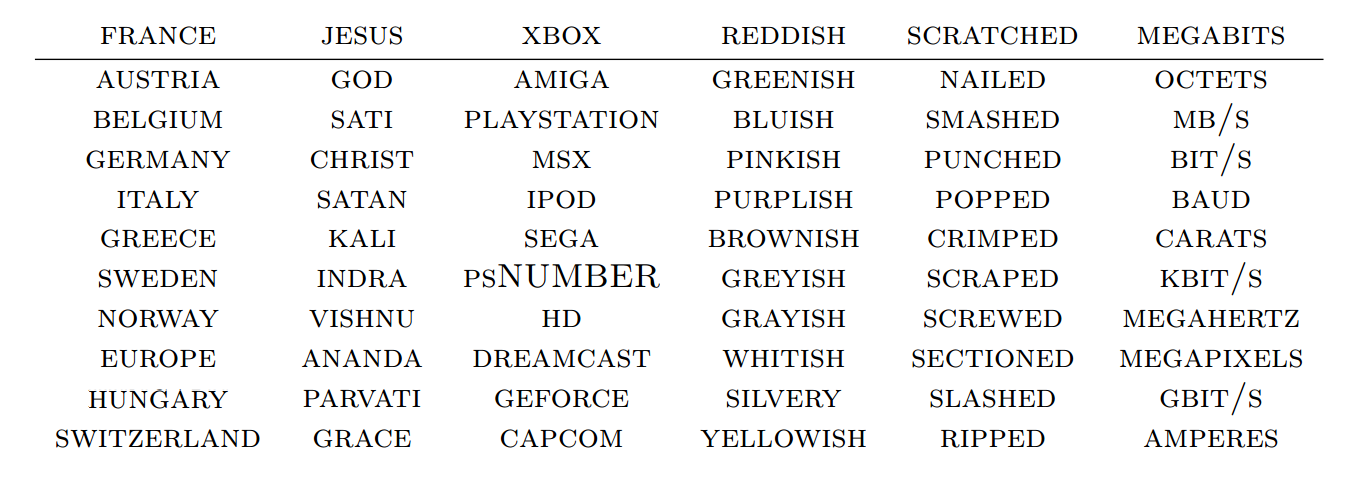
\includegraphics[width = 100mm]{weanalogies.png}
	\caption{Parole con vettori simili}
	\label{similarwords}
\end{figure}

Da questo potrebbe sembrare necessario osservare esempi relativi ad ogni parola per permetterci di generalizzarla. Comprendi tutte le parole che hai già visto, ma non hai già visto tutte le frasi che riesci a capire. Questo è l’approccio delle reti neurali.

\paragraph{Analogie}Il word embedding mostra un altra proprietà interessante anche se molto controversa: le analogie. Le analogie tra parole sembrano essere nascoste nella differenza dei loro rispettivi vettori \cite{Mikolov13}. 
\begin{equation}
  W\left ( "woman" \right ) -  W\left ( "man" \right ) \simeq W\left ( "aunt" \right ) -  W\left ( "uncle" \right )
\end{equation}
Da questo si evince che c’è una correlazione tra delle parole e le rispettive forme del genere opposto in quanto appariranno in contesti simile, differenti solo per alcuni dettagli come pronomi o articoli. Stessa cosa per tra singolare e plurale \cite{Mikolov13}.
\begin{figure}[htb]
	\centering
	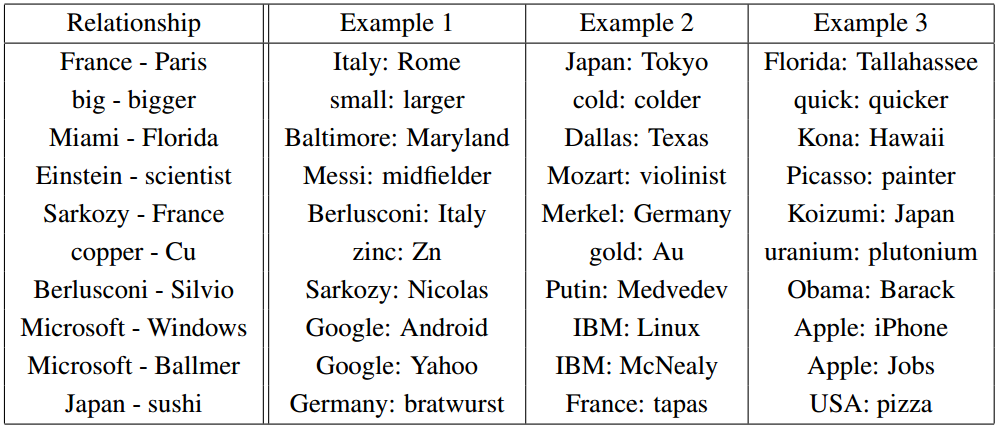
\includegraphics[width = 100mm]{weanalogies2.png}
	\caption{Alcuni esempi di analogie}
	\label{analogies}
\end{figure}
Queste proprietà possono essere considerate effetti collaterali. Non si è cercato di far apprendere il modello in modo da avere parole simili vicine fra loro. Questo sembra essere un punto di forza delle reti neurali nell’apprendere features che rappresentano bene i dati in modo automatico. invece di apprendere un rappresentazione dei dati specifica ed usarla per diversi task, è possibile apprendere un metodo per associare diversi tipi di dati in una singola rappresentazione. Queste tecniche sono note come transfer learning, metodi per applicare la conoscenza già appresa in contesti simili.
\\\\
Un esempio può essere il word embedding di parole linguaggi diversi. Dato che parole simili saranno associate a vettori simili, parole con significato simile in una lingua e nell’altra finiranno vicine tra loro, così come i loro sinonimi. È possibile notare che anche parole di cui non si conosceva la traduzione o che avessero significati simili, sono finite vicine tra loro \cite{Zou13}.
\begin{figure}[htb]
	\centering
	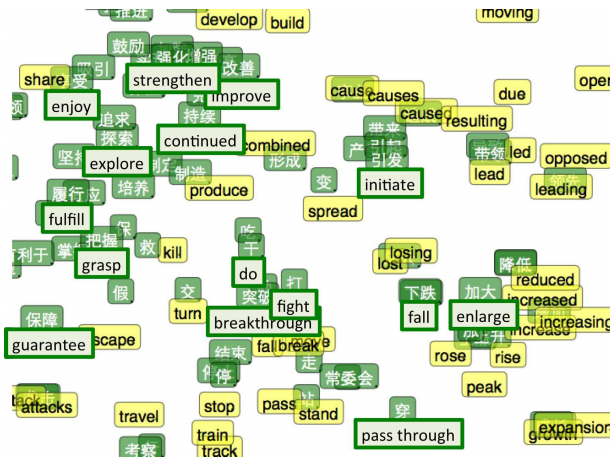
\includegraphics[width = 100mm]{englishchinese.png}
	\caption{Visualizzazione con t-SNE di un word embedding bilingua. }
	\label{englishchinese}
\end{figure}

\subsection{Word2vec}
Un algoritmo molto famoso di word embedding è il recente word2vec. L’algoritmo usa i documenti per far apprendere una rete neurale, massimizzando la probabilità condizionata del contesto data una parola, applicando il modello appreso ad ogni parola per ricavare il vettore corrispondente e calcolando il vettore della frase facendo la media dei vettori delle parole, costruisce la matrice di similarità delle frasi ed usa PageRank per classificare le frasi nel grafo.
\begin{equation}
   arg\max_{\theta} \prod_{\left ( w, c \right ) \in D} p\left ( c|w; \theta \right )
\end{equation}
L’obiettivo è di ottimizzare il parametro $ \left (\theta \right )$ massimizzando la probabilità condizionata del contesto $\left ( c \right )$ data la parola $\left ( w \right )$. $D$ è l’insieme di tutte le coppie $\left ( w, c \right )$. 
Per esempio: “ho mangiato un \underline{\hspace{1cm}}  al McDonald ieri sera”, molto probabilmente restituirà “Big Mac”.
\\\\
Applicare il modello di ogni parola per ottenere il suo vettore corrispondente (Figura \ref{2w2v})
\begin{figure}[htb]
	\centering
	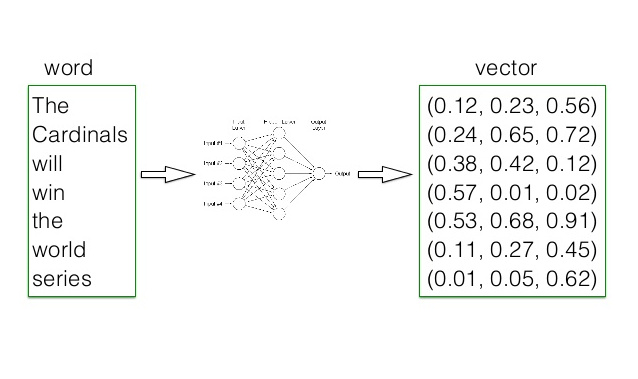
\includegraphics[width = 100mm]{2w2v.jpg}
	\caption{Vettori corrispondenti alle parole}
	\label{2w2v}
\end{figure}
\\\\
Calcolare il vettore delle frasi facendo la media del vettore delle loro parole (Figura \ref{3w2v})
\begin{figure}[htb]
	\centering
	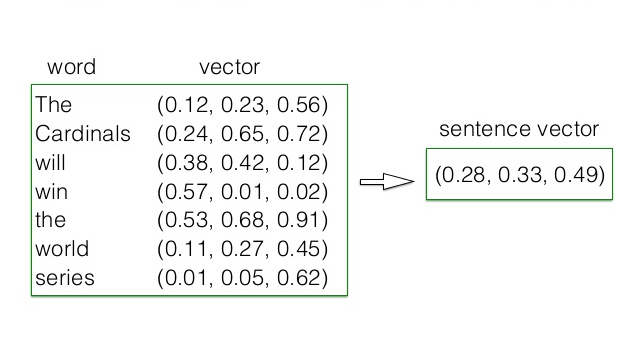
\includegraphics[width = 100mm]{3w2v.jpg}
	\caption{Vettori corrispondenti alle frasi}
	\label{3w2v}
\end{figure}
\\\\
Costruire la matrice di similarità delle frasi (Figura \ref{4w2v})
\begin{figure}[htb]
	\centering
	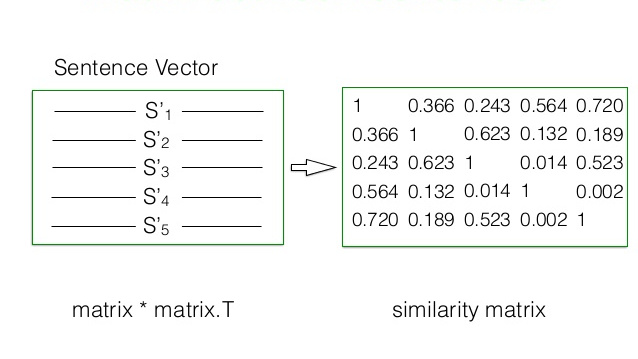
\includegraphics[width = 100mm]{4w2v.jpg}
	\caption{Matrice di similarità}
	\label{4w2v}
\end{figure}
\\\\
Infine usare PageRank par classificare le frasi nel grafo.
 (Figura \ref{5w2v})
\begin{figure}[htb]
	\centering
	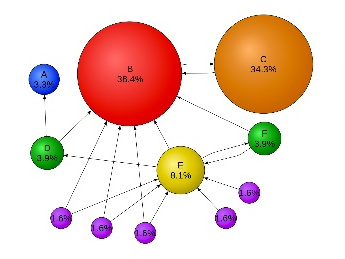
\includegraphics[width = 100mm]{5w2v.jpg}
	\caption{Assegna uno "score" utilizzando Pagerank}
	\label{5w2v}
\end{figure}

Word2vec è una rete neurale a due layer, sebbene non sia profonda (deep neural network) come spesso definita, trasforma il testo in modo che altre reti neurali possano comprenderlo. Prende in input un corpus di documenti e genera un insieme di vettori: feature vectors per ogni parola del corpus. I vettori restituiti sono rappresentazioni numeriche del contesto della singola parola. 
\\\\
Dati abbastanza dati, utilizzo e contesti, word2vec può apprendere rappresentazioni delle parole altamente accurate, basate sulle apparizioni della parola nei diversi contesti. Queste rappresentazioni possono essere usate per trovare associazioni fra parole o per raggruppare documenti e classificarli per argomento. La similarità fra i vettori può essere misurata attraverso la coseno similarità, dove nessuna similarità è espressa come un angolo di 90 gradi, mentre una similarità totale è data  da un angolo di 0 gradi tra i vettori. Ad esempio il vettore relativo a “Sweden” è uguale al vettore “Sweden” mentre il vettore “Norway” ha una distanza di similarità di $0.760124$.
\\\\
Word2vec può apprendere rappresentazioni principalemente in due modi, o usando il contesto per predire la parola data (metodo conosciuto come “continous bag of word”, o \textbf{CBOW}), o usando una parola per predire il contesto (\textbf{skip-gram}).

\section{Random Walk}
In matematica, un Random Walk è la formalizzazione dell'idea di prendere passi successivi in direzioni casuali. Matematicamente parlando, è il processo stocastico più semplice, il processo markoviano. Qui sono utilizzati per ricavare percorsi pseudo casuali da attraversamento del grafo del web per ottenere sequenze di URL collegati semanticamente.
\\\\
In una passeggiata aleatoria monodimensionale si studia il moto di una particella puntiforme vincolata a muoversi lungo una retta nelle due direzioni consentite. Ad ogni movimento essa si sposta (a caso) di un passo a destra (con una probabilità fissata $\ p$) o a sinistra con una probabilità $\ 1-p$, ed ogni passo è di lunghezza uguale e indipendente dagli altri.
\begin{figure}[htb]
	\centering
	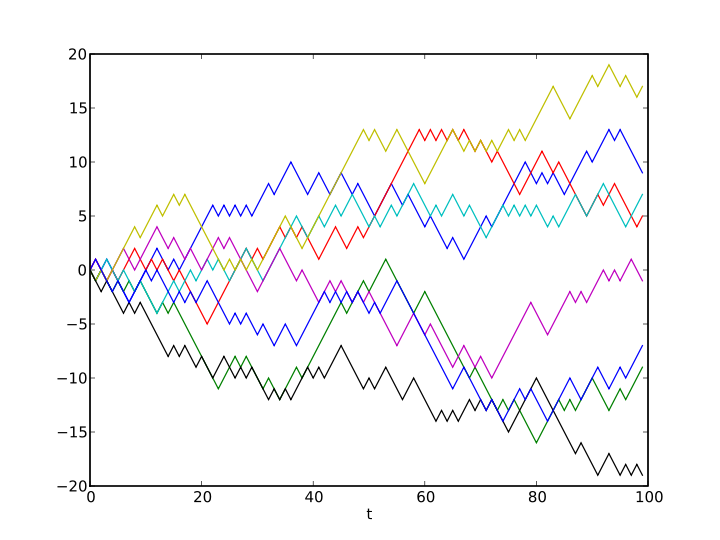
\includegraphics[width = 100mm]{randomwalkonedim.png}
	\caption{Rappresentazione visuale di 8 random walk monodimensionali. }
	\label{englishchinese}
\end{figure}
\\\\
In una passeggiata aleatoria bidimensionale si studia il moto di una particella vincolata a muoversi sul piano spostandosi casualmente ad ogni passo a destra o a sinistra con probabilità $\frac{1}{2}$, verso l'alto o verso il basso con probabilità $\ p=\frac{1}{2}$. In pratica ad ogni passo può compiere un movimento lungo una delle quattro diagonali con probabilità $\frac{1}{4}$. Ci si chiede con che probabilità la particella tornerà al punto di partenza.
\begin{figure}[htb]
	\centering
	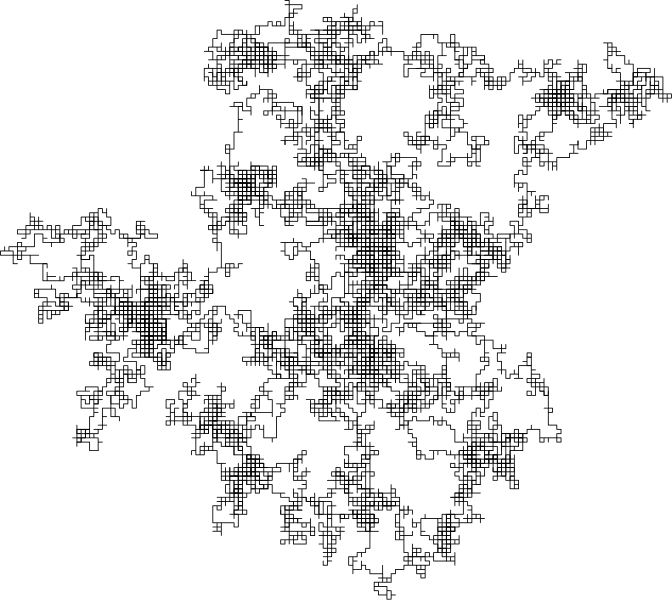
\includegraphics[width = 100mm]{randomwalktwodim.png}
	\caption{Rappresentazione visuale di un random walk di 25.000 passi su due dimensioni. }
	\label{englishchinese}
\end{figure}
\\\\
Queste passeggiate aleatorie possono trovare effettivi riscontri in natura come il traiettoria percorso da una particella in un liquido o in un gas, il tragitto di un animale affamato o anche il prezzo di un titolo fluttuante o la situazione finanziaria di un giocatore d'azzardo. Tutti questi esempi possono essere espressi come random walk, anche se in natura potrebbero non essere veramente casuali.
\\\\
Un popolare modello di random walk è quello su un reticolo regolare, dove ad ogni passo si segue un determinato percorso basandosi su una qualche distribuzione di probabilità. Nel caso più semplice si può solo “saltare” sul sito vicino. In un semplice random walk simmetrico in un reticolo localmente finito, le probabilità di saltare su ognuno dei siti vicini è la stessa.
\\\\
Per definire un random walk formalmente, prese indipendenti variabili casuali $ Z_1, Z_2, Z_3, $ \dots dove ogni variabile è o 1 o -1, con una probabilita del 50\% per ognuno dei due casi, e dato 
\begin{equation}
  S_0 = 0
\end{equation}
\begin{equation}
  S_n = \sum_{j=1}^{n} Z_j
\end{equation}
  
la serie $\left \{ S_n \right \} $ è chiamata random walk semplice in $\mathbb{Z}$.
\\\\
Si consideri un attraversatore casuale della rete (random surfer) che, partendo da un pagina web, esegue un passo alla volta in questo modo: ad ogni iterazione, dalla pagina corrente, procede verso una pagina a caso tale che esiste un link che dalla pagina corrente punta a questa.
\\\\
Procedendo da pagina a pagina, visiterò alcuni nodi, più spesso di altri; intuitivamente, saranno nodi con molti link entranti da altri nodi frequentemente visitati.
\\\\
Ci sono alcuni problemi. Che succede se si arriva ad una pagina che non ha link in uscita? In questo caso è necessario introdurre un’altra operazione: il teletrasporto. In questa operazione l’attraversatore casuale salta dal nodo corrente ad un qualsiasi altro nodo sulla rete.
Se $N$ è il numero totale dei nodi nel grafo, l’operazione di teletrasporto porta l’attraversatore verso ogni nodo con probabilità $\frac{1}{N}$. Potrebbe anche trasportarsi sulla posizione corrente con probabilità di $\frac{1}{N}$. Questa operazione è chiamata quando si arriva ad un non senza nodi in uscita o con una probabilità$\ d$ data, con$\ 0 < d < 1$.


\section{Clustering}
Sono un insieme di tecniche di analisi multivariata dei dati volte alla selezione e raggruppamento di elementi omogenei in un insieme di dati \cite{tryon}. Le tecniche di clustering si basano su misure relative alla somiglianza tra gli elementi. In molti approcci questa similarità (o dissimilarità) è concepita in termini di distanza in uno spazio multidimensionale. La bontà delle analisi ottenute dagli algoritmi di clustering dipende molto dalla scelta della metrica, e quindi da come è calcolata la distanza. Gli algoritmi di clustering raggruppano gli elementi sulla base della loro distanza reciproca, e quindi l'appartenenza o meno ad un insieme dipende da quanto l'elemento preso in esame è distante dall'insieme stesso dividendo gli elementi in più cluster(soft/fuzzy clustering) o in un solo cluster(hard cluster).
Le tecniche di clustering si possono basare principalmente su due "filosofie":
partizionale e gerarchico.

\subsubsection{Partizionale}
Gli algoritmi di clustering di questa famiglia creano una partizione delle osservazioni minimizzando una certa funzione di costo:
\begin{equation}
  \sum_{j=1}^{k} E\left ( C_j \right )
\end{equation}
dove $ k$ è il numero desiderato di cluster, $ C_j$ è il j-esimo cluster e $ E : C \to \mathbb{R^+}$ è la funzione di costo associata al singolo cluster. L'algoritmo più famoso appartenente a questa famiglia è il k-means, chiamato così da MacQueen nel 1967 \cite{MacQueen67}.

\subsubsection{Gerarchico}
Nel clustering gerarchico, invece, è necessario individuare il cluster da suddividere in due sottogruppi. Per questa ragione sono necessarie funzioni che misurino la compattezza del cluster, la densità o la distanza dei punti assegnati ad un cluster. Le funzioni normalmente utilizzate nel caso divisivo sono:
\paragraph{Single-link proximity}
Calcola la distanza tra i due cluster come la distanza minima tra elementi appartenenti a cluster diversi:
\begin{equation}
  D\left ( C_i, C_j \right ) = \min_{x \in C_i, y \in C_j} d\left ( x, y \right )
\end{equation}

\paragraph{Average-link proximity}
Questa funzione calcola la distanza tra i due cluster come la media delle distanze elementi:
\begin{equation}
  D\left ( C_i, C_j \right ) = \frac{1}{|C_i||C_j|}\sum_{x \in C_i, y \in C_j} d\left ( x, y \right )
\end{equation}

\paragraph{Complete-link proximity}
Questa funzione valuta la distanza massima tra due punti interni ad un cluster. Tale valore è noto anche come 'diametro del cluster': più tale valore è basso, più il cluster è compatto:
\begin{equation}
  D\left ( C_i, C_j \right ) = \max_{x \in C_i, y \in C_j} d\left ( x, y \right )
\end{equation}

\paragraph{Distanza tra centroidi}
Questa funzione valuta la distanza massima tra due punti interni ad un cluster. Tale valore è noto anche come 'diametro del cluster': più tale valore è basso, più il cluster è compatto:
\begin{equation}
  D\left ( C_i, C_j \right ) = d\left ( \hat{c_i}, \hat{c_j} \right )
\end{equation}


Nei casi precedenti, $ d\left ( x, y \right )$ indica una qualsiasi funzione distanza su uno spazio metrico.
\begin{figure}[htb]
	\centering
	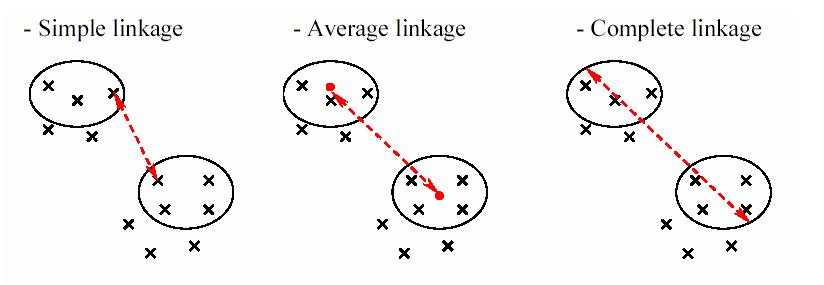
\includegraphics[width = 100mm]{linkages.jpg}
	\caption{Differenze fra i vari tipi di funzioni distanza}
	\label{linkages}
\end{figure}

\subsection{Graph Clustering}
Un grafo è una coppia ordinata $ G = (V, E)$ di insiemi, con $V$ insieme dei nodi ed $E$ insieme degli archi, tali che gli elementi di $E$ siano coppie di elementi da $V$ da $ E \subseteq V\times V$ segue in particolare che  $|E|\le |V|^2$.
\\\\
I grafi sono oggetti discreti che permettono di schematizzare una grande varietà di situazioni e di processi e spesso di consentirne delle analisi in termini quantitativi e algoritmici.
\\\\
Nello studio di reti complesse, è possibile trovare gruppi di nodi fortemente connessi, che possono essere raggruppati in comunità (potenzialmente sovrapposte). Questa disomogeneità di connessioni suggerisce che esiste una certa divisione naturale all’interno della rete. Nel caso particolare di strutture non sovrapposte, la ricerca di comunità implica la divisione della rete in gruppi di nodi con fortemente connessi internamente e connessioni sparse fra i gruppi.
Una definizione più generale è basata sul principio che coppie di nodi sono più probabilmente connessi se fanno parte della stessa comunità, e meno probabilmente connessi se non condividono la stessa comunità.
\\\\
Le comunità sono molto comuni all’interno delle reti. Le reti sociali includono gruppi di comunità che condividono la posizione, gli interessi, l’occupazione ecc. Essere in grado di individuare queste sotto-strutture all’interno di una rete può fornire indizi  su come come funziona la rete in considerazione o la topologia che influenza i nodi. Questi indizi possono essere utili per implementare algoritmi sui grafi. Molti metodi di community detection sono stati sviluppati con diversi livelli di successo.

\subsubsection{Minimum-cut method}
In questo metodo, la rete è divisa in un numero predeterminato di parti, generalmente della stessa grandezza, scelte in modo che il numero degli archi tra i gruppi è minimizzato. Questo metodo funziona bene in molte applicazioni per le quali è stato ideato, ma non è la scelta migliore per scovare comunità in reti generali, dato che troverà comunità indistintamente dal fatto che queste ci siano o meno e troverà solo un numero fissato di comunità.

\subsubsection{Hierachical-clustering}
Un altro metodo per scovare sotto-strutture conesse nelle reti viene effettuato tramite algoritmi di clustering gerarchico. Con questo approccio si definisce una misura di similarità fra coppie di nodi. Misure comunemente usate sono la coseno similarità, l’indice di Jaccard e la distanza di Hamming fra le righe della matrice di adiacenza. Poi i gruppi di nodi simili vengono raggruppati in comunità.

\subsubsection{Girvan-newman algorithm}
Un altro algoritmo molto utilizzato è quello di Girvan–Newman. Questo algoritmo identifica all’interno della rete, gli archi che uniscono community diverse e li rimuove, isolandole. L’identificazione di tali archi è effettuata applicando una misura nota della teoria dei grafi: la \textbf{betweenness centrality}. Questa assegna un valore ad ogni arco, che è alto tanto più l’arco è attraversato nel cammino più breve (geodesico) che collega due qualsiasi nodi della rete.
\begin{figure}[htb]
	\centering
	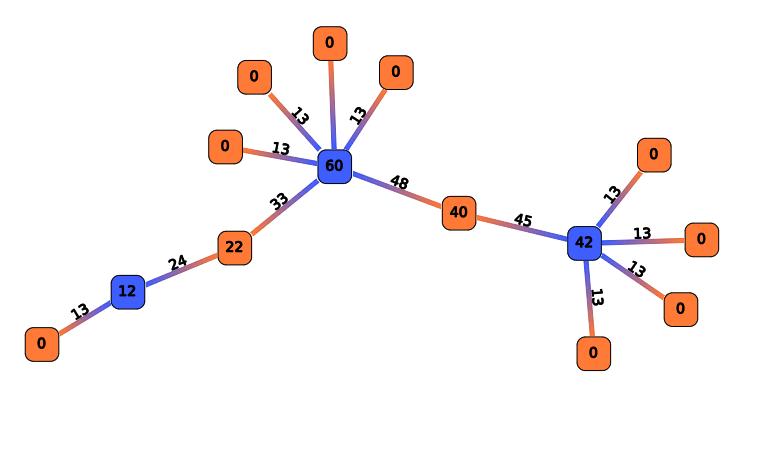
\includegraphics[width = 100mm]{betweenness.png}
	\caption{Betweenneess centrality score}
	\label{betweenness}
\end{figure}

\subsubsection{Modularity maximization}
La modularità è una misura che viene attribuita al grafo.  Questa compara la densità all’interno dei cluster con la densità fra di essi. Indica una certa divisione intrinseca e viene utilizzata per conoscere “quanto“ un grafo è separato.
\\\\
Nonostante i suoi svantaggi uno dei metodi più utilizzati per il community detection è la massimizzazione della modularità. Questo approccio scova strutture connesse tramite la ricerca della miglior divisione di una rete in modo che la modularità risulti massimizzata. 
\\\\
Dato che effettuare un confronto su tutte le possibili combinazioni è solitamente impraticabile, gli algoritmi di questa famiglia si basano su metodi di ottimizzazione approssimati quali algoritmi greedy, cioè che cercano di ottenere una soluzione ottima da un punto di vista globale attraverso la scelta della soluzione considerata migliore ad ogni passo locale. Un famoso approccio di questo tipo è il metodo Louvain, che ottimizza le community locali iterativamente, fin quando la modularità globale non può più essere migliorata. 
\\\\
L’accuratezza di questi algoritmi, comunque, è dibattuta, in quanto è stato dimostrato che molte volte fallisce nell’individuare cluster più piccola di una certa soglia, dipendente dalla grandezza della rete. 
\begin{figure}[htb]
	\centering
	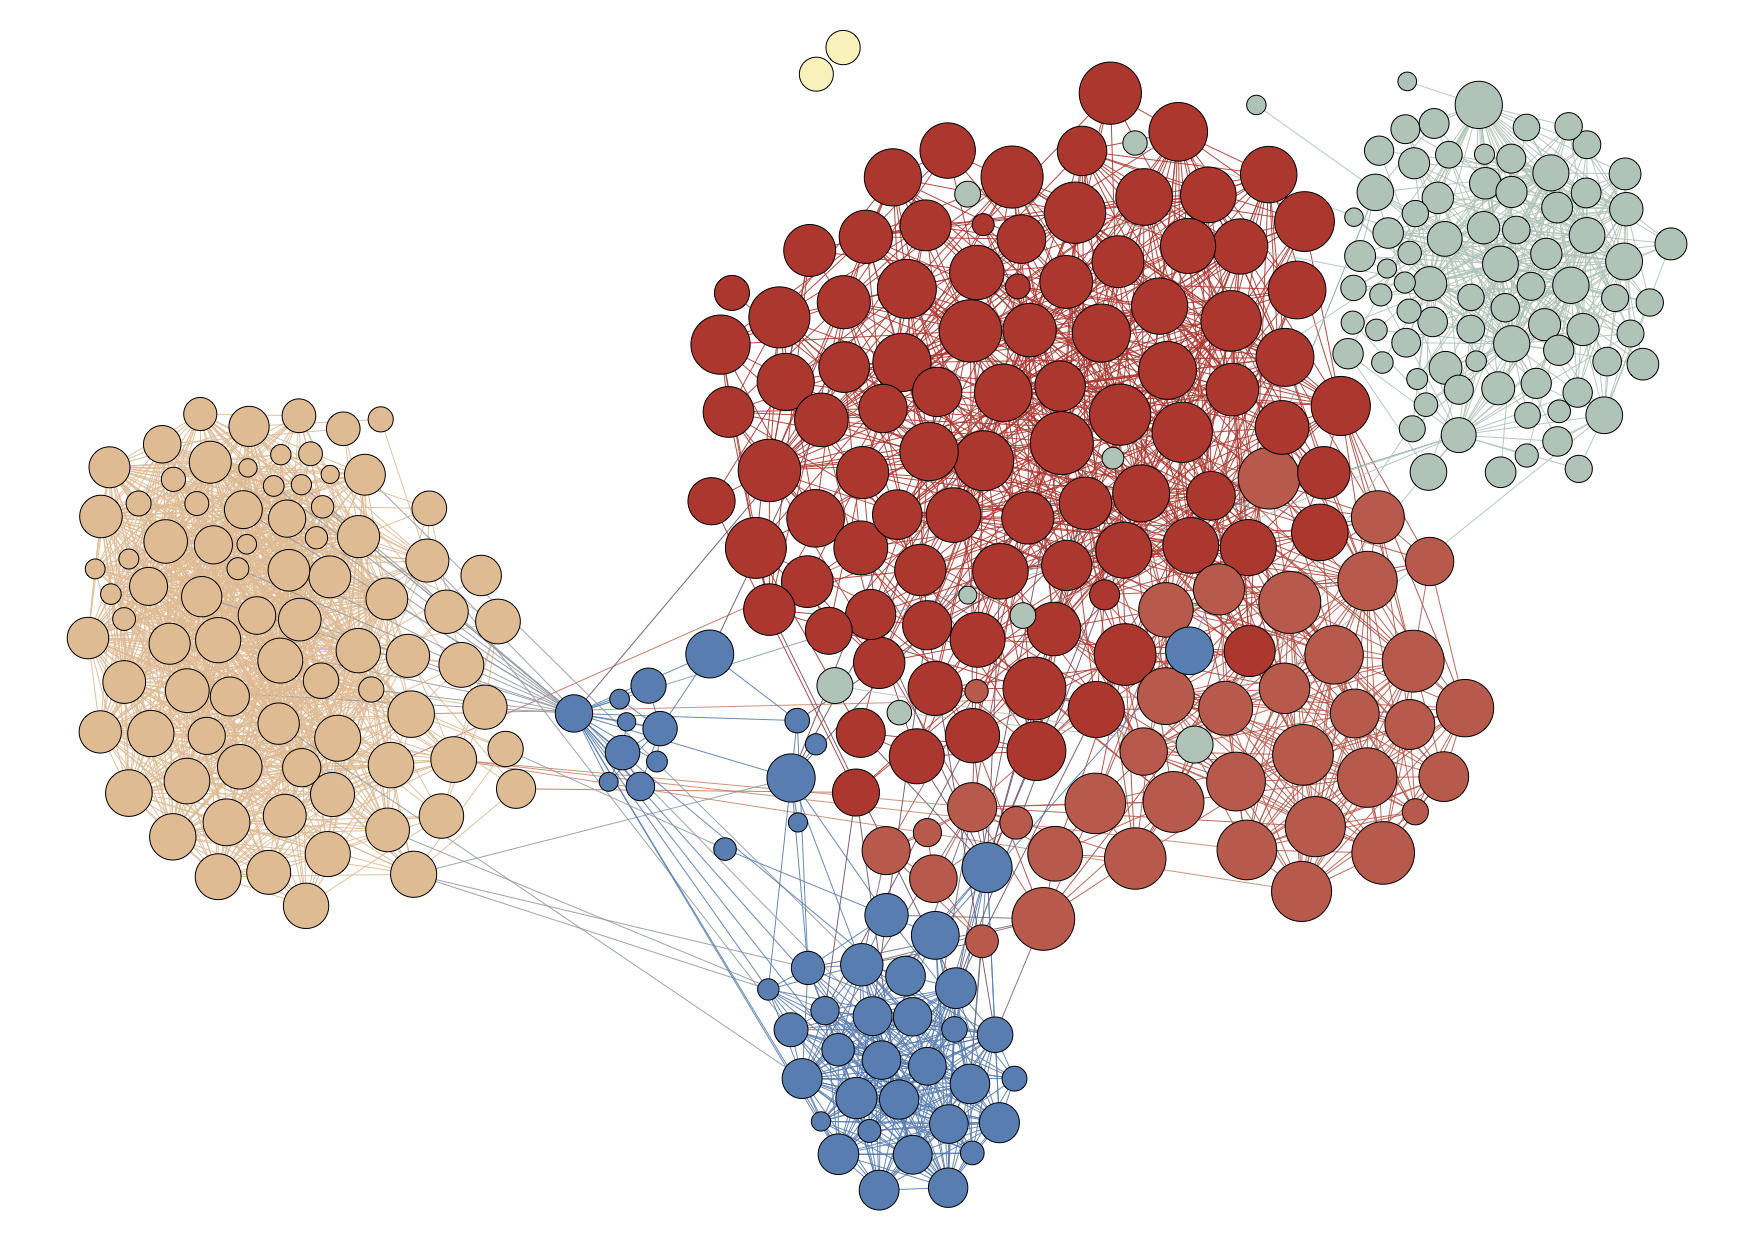
\includegraphics[width = 100mm]{modularity.png}
	\caption{Modularity score}
	\label{modularity}
\end{figure}
\subsubsection{Clique-based methods}
Le cricche (cliques) sono sottografi dove ogni nodo è collegato con ogni altro nodo nella cricca. Dato che i nodi non possono essere più connessi di così, non è sorprendente che ci siano molti metodi in community detection che si basano su questo approccio. È da notare che dato che un nodo può far parte di più di una cricca, quindi può far parte di più community contemporaneamente, questi metodi restituiscono strutture sovrapposte. 
Un approccio consiste nel trovare cricche tali che non siano sottografi di altre cricche. Un classico algoritmo per scovare tali strutture è quello di Bron-Kerbosch.



\subsection{Vector Clustering}
Gli algoritmi di clustering in uno spazio vettoriale seguono un altro approccio. Qui viene preso in considerazione la vicinanza (o la distanza) degli elementi rappresentati come punti su un iperpiano. Il feature vector associato può avere grandi dimensioni e può essere ottenuto utilizzando diverse metodologie, dipendentemente dal tipo di dato eleborato. 

\subsubsection{Hierarchical Clustering}
Anche qui il clustering gerarchico è molto utilizzato, seguendo un approccio divisivo (top-down) o agglomerativo (bottom-up), l’idea è quella di unire (o separare) elementi in base alla loro vicinanza, seguendo uno degli approcci già descritti, costruendo così una struttura chiamata dendrogramma che raggruppa gli elementi ad ogni livello. La differenza risiede nel come viene calcolata la distanza.

\subsubsection{Centroid-based clustering}
Nell’approccio basato sui centroidi, i cluster sonorappresentati da un vettore centrale, che non è neccessariamente un membro del dataset. Quando il numero dei cluster è prefissato ad un numero k, la seguente definizione formale può essere applicata: vengono definiti k centroidi e si prosegue assegnando ogni elemento al centroide più vicino, tale che il quadrato delle distanze dal cluster è minimizzato. Molti algoritmi di questa famiglia richiedono che il parametro k sia stabilito in precedenza, che è il loro più grande svantaggio. Inoltre solitamente vengono trovati cluster di grandezza simile, dato che verrà assegnato un elemento al centroide più vicino. Questi metodi partizionano lo spazio dei dati in una struttura conosciuta come diagramma di Voronoi.
\begin{figure}[htb]
	\centering
	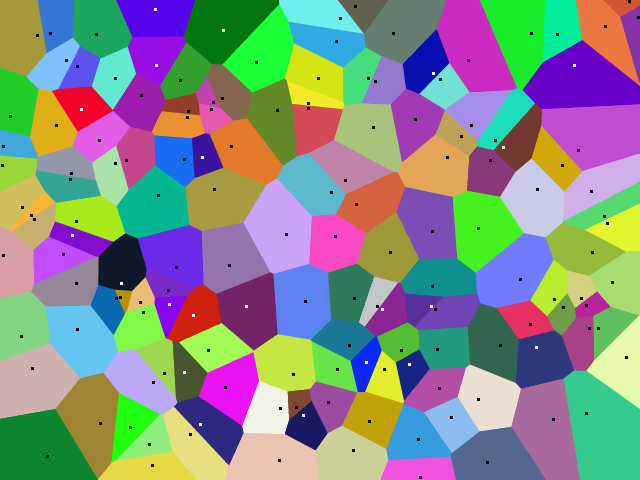
\includegraphics[width = 100mm]{voronoi.png}
	\caption{Diagramma di Voronoi}
	\label{voronoi}
\end{figure}
Nonostante questo, rimangono tra degli approcci più utilizzati ed efficaci. Da notare anche la somiglianza concettuale con l’algoritmo di classificazione KNN (k nearest neighbor).

\subsubsection{Distribution-based clustering}
Il raggruppamento avviene analizzando l'intorno di ogni punto dello spazio. In particolare, viene considerata la densità di punti in un intorno di raggio fissato. Si basano sul considerare collegati due punti che si trovano all’interno di una certa distanza limite.
I cluster sono definiti come aree con più alta densità rispetto al resto del dataset. Elementi in un area meno denso sono spesso considerati rumore, quindi come non facenti parte di nessun cluster.
\\\\
Uno degli svantaggi di questi algoritmi è che si aspettano un certo tipo di densità comune a tutti i cluster. Inoltre non eccellono nel scovare cluster presenti in molti dati del mondo reale.

\subsubsection{Document Clustering}
Agisce sempre nello spazio vettoriale, si differenzia principalmente nelle operazioni di pre-processing finalizzate ad ottenere un feature vector utilizzabile. 
Un approccio efficace consiste nel rappresentare i documenti come vettori dove ogni dimensione rappresenta la frequenza di occorrenza di una parola del vocabolario, un insieme di parole precedentemente costruito utilizzando tutte le parole del corpus. 
\begin{figure}[htb]
	\centering
	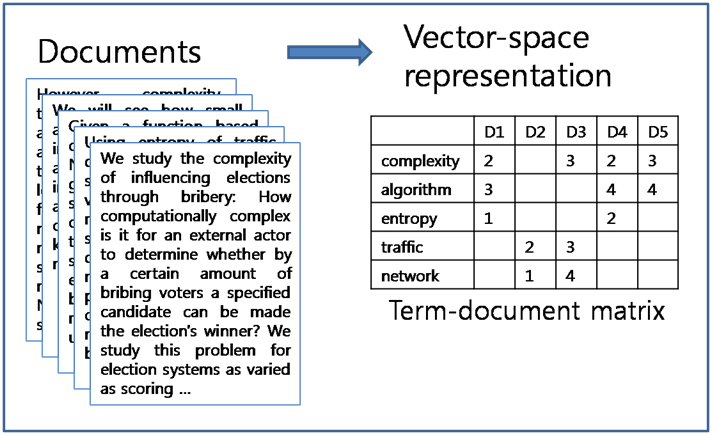
\includegraphics[width = 100mm]{tdm.png}
	\caption{Matrice termini-documenti. Ogni riga rappresenta un singolo termine ed ogni colonna rappresenta un singolo documento}
	\label{tdm}
\end{figure}

\paragraph{Term-Frequency (TF)}misura quante volte un termine appare in un documento. Dato che ogni documento ha lunghezza differente, è possibile che un termina possa apparire molte più volte nei documenti più lunghi che in quelli più corti. Quindi può essere necessario  dividere la frequenza dei termini per documenti aventi la stessa lunghezza.

\paragraph{Inverse-Document-Frequency (IDF)}un altro aspetto da considerare è a frequenza di un termine in un documento relativamente alla sua presenza globale in tutto il corpus. Tenendo in considerazione solo la frequenza di occorrenza tutti i termini sono considerati ugulamente importanti. Termini che appaiono molte volte in un documento ma meno volte in tutto il corpus potrebbero essere molto più significativi per quel specifico documento e portare molta più informazione, quindi tendono ad essere più importanti. Così come i termini che appaiono molte volte in tutti i dcoumenti del corpus sono spesso poco rilevanti e considerati inutili (stopwords).
\begin{equation}
	idf_i = \log \frac{|D|}{|\left \{ d : t_i \in d \right \}|}
\end{equation}
dove $ |D| $ è il numero di documenti nella collezione, mentre il denominatore è il numero di documenti che contengono il termine $t_i$.
Tale funzione aumenta proporzionalmente al numero di volte che il termine è contenuto nel documento, ma cresce in maniera inversamente proporzionale con la frequenza del termine nella collezione. L'idea alla base di questo comportamento è di dare più importanza ai termini che compaiono nel documento, ma che in generale sono poco frequenti.
\\\\
Altre tecniche utilizzate nel clustering sui documenti sono
\paragraph{LSI} il \textbf{Latent Semantic Indexing} è un metodo di indicizzazione e reperimento che usa una tecnica matematica chiamata decomposizione a valori singolari (SVD) per identificare pattern nelle relazioni tra i termini e i concetti contenuti in una colezione non strutturata di testo. La LSI è basata sul principio che parole che sono usate nello stesso contesto tendono ad avere significato simile. Chiamata così per la sua abilità di correlare semanticamente termini correlati che sono nascosti (latenti) in grandi collezioni testuali. La SVD può venire troncata per task di dimensionality reduction, in modo da diminuire la dimensione del vettore mantenendo comunque il significato.

\paragraph{Coseno similarità} una euristica per la misurazione della similitudine tra due vettori effettuata calcolando il coseno tra di loro. Dati due vettori di attributi numerici, $A$ e $B$, il livello di similarità tra di loro è espresso utilizzando la formula
\begin{equation}
	similarity = \cos \theta = \frac{A\cdot B}{||A||||B||}
\end{equation}
In base alla definizione del coseno, dati due vettori si otterrà sempre un valore di similitudine compreso tra $-1$ e $+1$, dove $-1$ indica una corrispondenza esatta ma opposta (ossia un vettore contiene l'opposto dei valori presenti nell'altro) e $+1$ indica due vettori uguali.
Nel caso dell'analisi dei testi, poiché le frequenze dei termini sono sempre valori positivi, si otterranno valori che vanno da 0 a $+1$, dove $+1$ indica che le parole contenute nei due testi sono le stesse (ma non necessariamente nello stesso ordine) e $0$ che non c'è nessuna parola che appare in entrambi.


\section{Data Visualization}
Un nota sulla visualizzazione dei dati, campo in crescita data la corrispondente crescita su economie basate sull’informazione e sulla crescita dei dati generati (big data) portata avanti anche da campi relativamente nuovi nel campo dell’analisi dei dati, come Business Analytics, Business Intelligence, Data Science etc.
\\\\
Tale disciplina è indirizzata a comunicare informazioni in modo chiaro e comprensibile, attraverso grafici, tabelle, diagrammi ecc. La visualizzazione può spesso aiutare ad analizzare e ragionare sui dati, rendendo dati complessi molto più accessibili ed usabili.
\begin{figure}[htb]
	\centering
	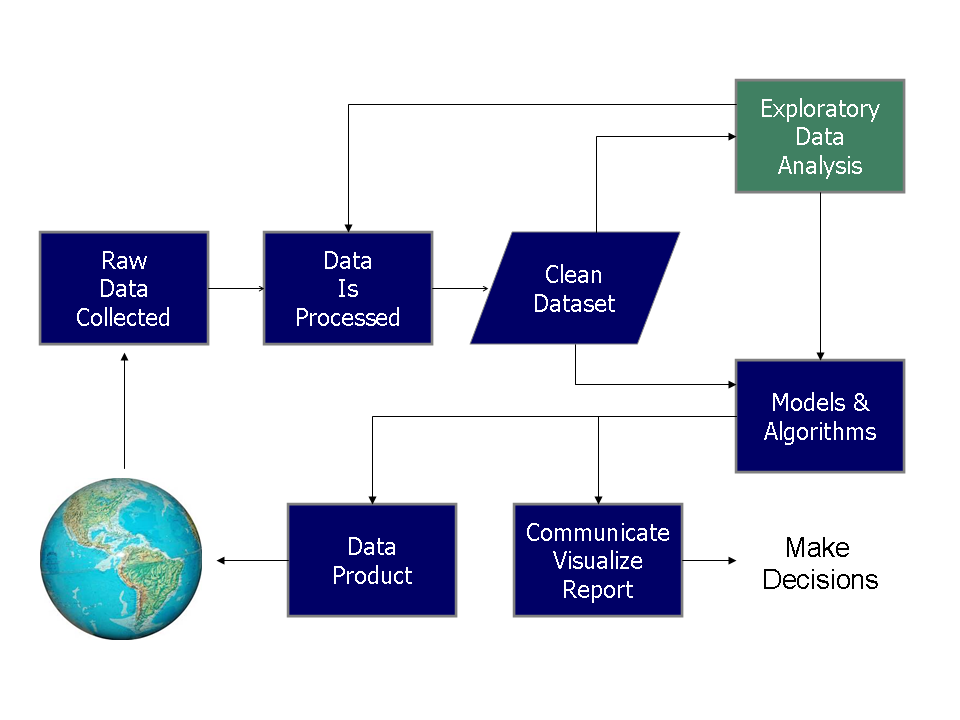
\includegraphics[width = 100mm]{datavisualization.png}
	\caption{La visualizzazione dei dati è un passo fondamentale nell'analisi dei dati.}
	\label{datavisualization}
\end{figure}

